\subsection{Les logs}

Le système de log est un module  connecté au réseau, chaque joueur doit donc recevoir les action effectué par les autre joueurs.
Pour ce faire, ce système est décomposé en 3 partis,
le \textit{LogClient}, le \textit{LogServer} et le \textit{LogGui},
cette dernière partie ne s'occupant que de l'affichage.

Lorsque qu'un joueur effectue une action (ajout, déplacement ou suppression d'un sprite), le gestionnaire de carte informe le gestionnaire de log a travers le \textit{LogClient}.
Celui ci permet, avec le \textit{LogServer} la communication des différentes interface de jeu.
Le \textit{LogServer} reçoit les information des différents \textit{LogClient} et les réexpédies à tous les clients.
Une fois cela fait, les \textit{LogClient} qui reçoivent maintenant l'information de tous les joueurs peuvent, par le biais du \textit{LogGui} afficher les differentes action dans un widget prévue à cet effet.

\begin{figure}[h!]
    \centering
    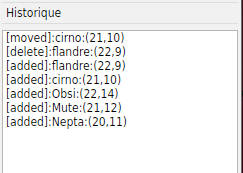
\includegraphics[scale=0.7]{img/log.png}
    \caption{historique}
    \label{fig:log}
\end{figure}